\section{WCET Analysis}
\label{sec:monitoring_wcet.wcet}

\subsection{Analysis Assumptions}

Our WCET analysis focuses on the interaction between the main core and the
monitoring core through a FIFO with an assumption that each core has its own
memory. Therefore, there is no interference between the two cores on memory
accesses. This configuration applies for typical multi-core embedded
microprocessors or a small monitor with a dedicated memory that is attached to
a large core. The main core is assumed to not exhibit timing anomalies. This is
required so that the worst-case monitoring stall cycles can be assumed to
produce the WCET on the main core.  We do not make any other assumptions on the
microarchitecture of each processing core. However, we assume that the WCET of
a main task and a monitoring task on the given processing cores can be
estimated individually using traditional WCET techniques.

\subsection{Implicit Path Enumeration}
\label{sec:monitoring_wcet.wcet.ipet}

Most of the WCET analysis techniques today rely on an integer linear
programming (ILP) formulation that is
obtained from implicit path enumeration techniques (IPET) \cite{li-ipet-dac95}.  In
this method, a program is converted to a control flow graph (CFG). From the
control flow graph, an ILP problem is formulated that seeks to maximize
\begin{align*}
  t = \sum_{B \in \mathcal{B}_{CFG}}{N_B \cdot c_{B,max}}
\end{align*} 
where $\mathcal{B}_{CFG}$ is the set of basic blocks in the control flow graph.
$N_{B}$ is the number of times block $B$ is executed and $c_{B,max}$ is the
maximum number of cycles to execute block $B$. The maximum value of $t$ is the
WCET of the task.  To account for the fact that only certain paths in the graph
will be executed, a set of constraints are placed on $N_{B}$. For example, on a
branch, only one of the branches will be taken on each execution of the block.
A variable can be assigned to each edge corresponding to the number of times
that edge is taken.  The number of times edges out of the block are taken must
equal the number of times the block is executed.  Similarly, the number of
times edges into the block are taken must equal the number of times the block
is executed. Various methods have been developed to create additional
constraints to convey other program behavior \cite{li-ipet-dac95,
wcetsurvey-tecs08}.

%% Why ILP?
Integer linear programming is an attractive optimization technique for this
problem because the solution found is a global optimum. In addition, many
aspects of program and architecture behavior can be described by adding
constraints to the ILP problem.  Several open source and commercial ILP solvers
exist which can solve the formulated ILP problem \cite{lpsolve, cplex}.  Thus,
in developing a method for estimating the WCET of parallel run-time monitoring,
we look to build upon this ILP framework.

%% Using worst case stalls in original WCET analysis to determine WCET with monitoring.
The IPET-based ILP formulation can be extended in a straightforward fashion to
incorporate run-time monitoring overheads if we have the maximum (worst-case)
monitoring stall cycles for each basic block by maximizing
\begin{align*}
  t = \sum_{B \in \mathcal{B}_{CFG}}{N_{B} \cdot (c_{B,max} + s_{B,max})}
\end{align*}
Here, $s_{B,max}$ represents the maximum number of cycles that block $B$ is
stalled due to monitoring. In this sense, the challenge in WCET analysis with
monitoring lies in determining $s_{B,max}$.  The rest of this section addresses
this problem.

\subsection{Sequential Monitoring Bound}
\label{sec:monitoring_wcet.wcet.sequential}

One way to determine a conservative bound on the worst-case monitoring stall
cycles is to consider sequential monitoring.  In sequential monitoring, the
monitoring task is run in-line with the main task on the same core rather than
in parallel. That is, after each instruction that would be forwarded, the
monitoring task is run on the main core before the main task resumes execution.
In this case, the WCET estimate can be obtained from a traditional method by
analyzing one program that contains both main and monitoring tasks.  The
resulting WCET can be considered as a simple bound for parallel monitoring
because it models the case where every forwarded instruction causes the main
core to stall.  However, this bound is extremely conservative as it does not
account for the FIFO buffering or the parallel execution of the monitoring
core. These features are critical to utilizing run-time monitoring techniques
while maintaining low performance overheads.

\subsection{FIFO Model}
\label{sec:monitoring_wcet.wcet.model}

To obtain tighter WCET bounds, we need to model the FIFO.  The main task can
continue its execution as long as a FIFO entry is available, but needs to stall
on a forwarded instruction if the FIFO is full. The WCET model needs to capture
the worst-case (maximum) number of entries in the FIFO at each forwarded
instruction and determine how many cycles the main task may be stalled due to
the FIFO being full. Here, we propose a mathematical model to express the load
in the FIFO and estimate the worst-case stalls.

% CFG, MFG
\begin{figure} 
  \begin{center} 
    \begin{subfigure}[Control flow graph.]{
      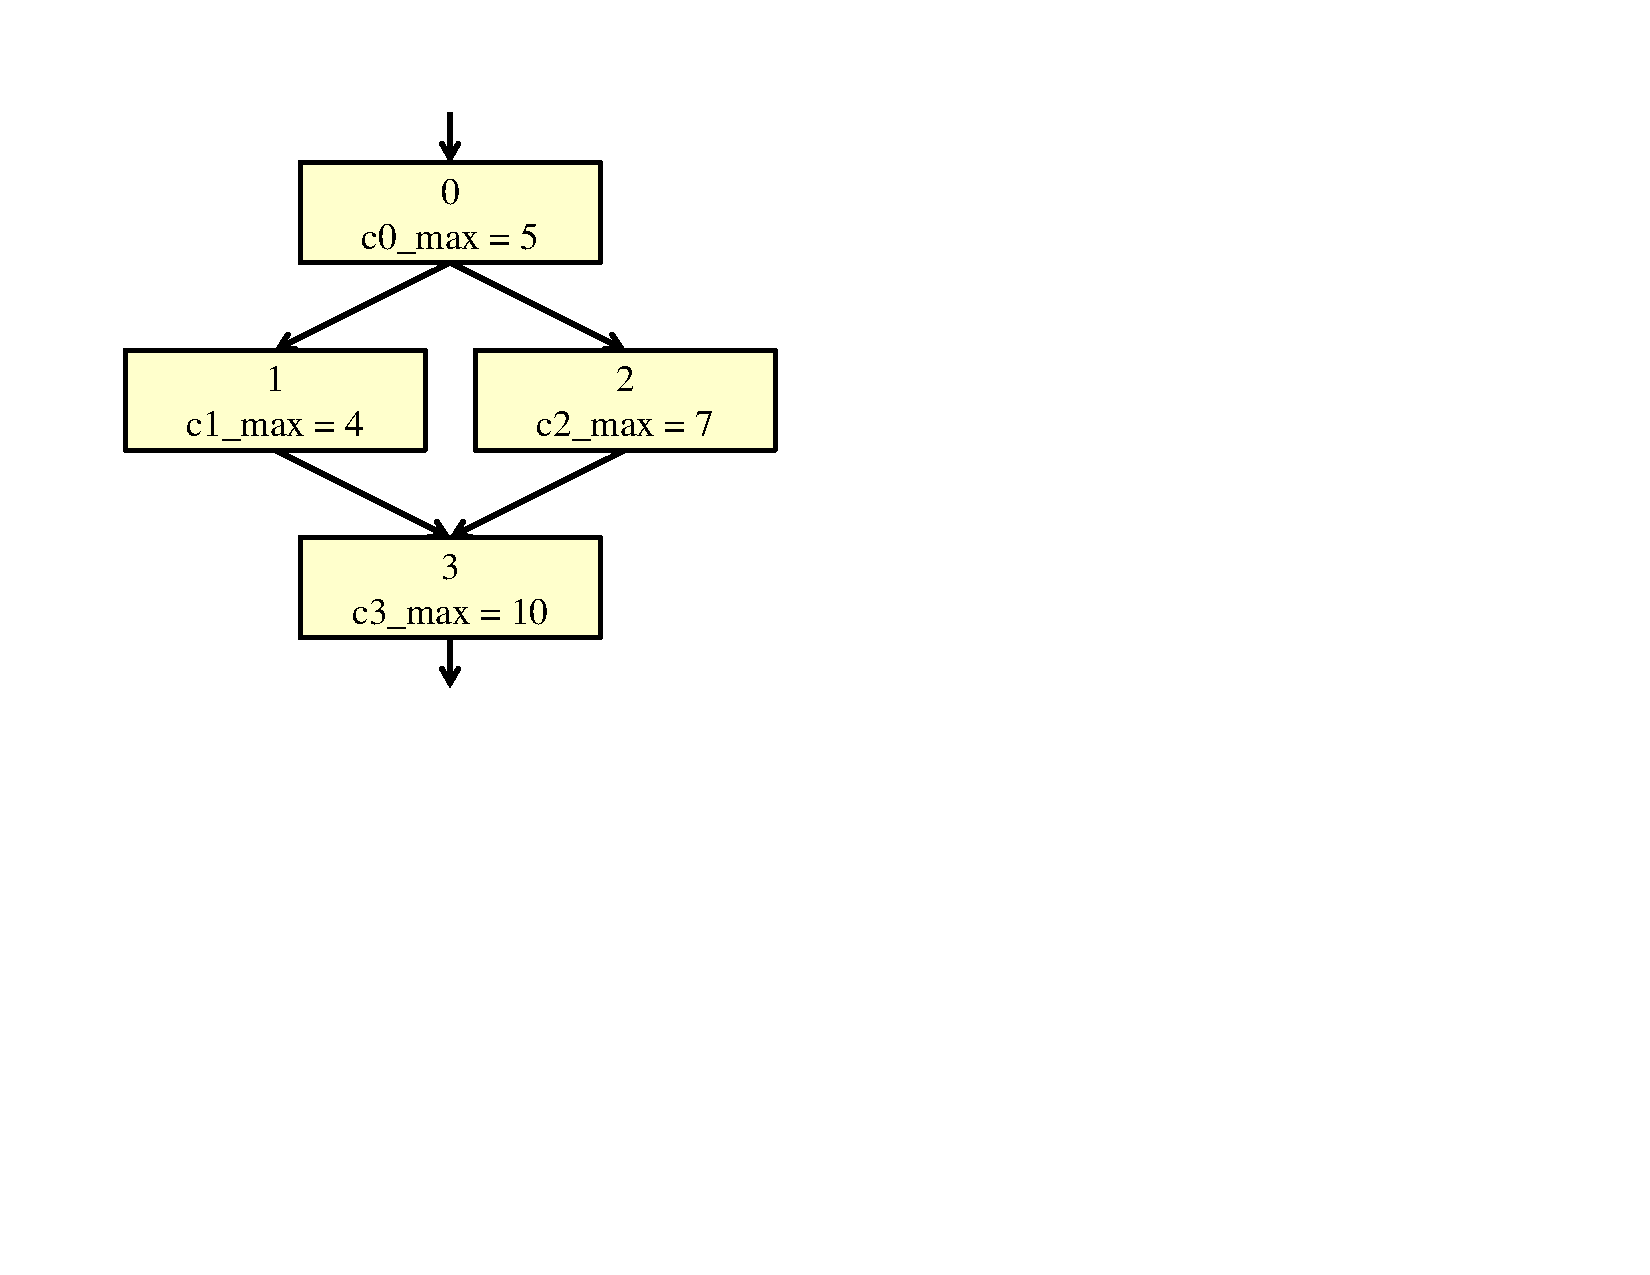
\includegraphics[width=2.9in]{monitoring_wcet/figs/cfg.pdf}
      \label{fig:monitoring_wcet.wcet.cfg} 
    }
    \end{subfigure}
    \hspace{-0.3in}
    \begin{subfigure}[Monitoring flow graph.]{
      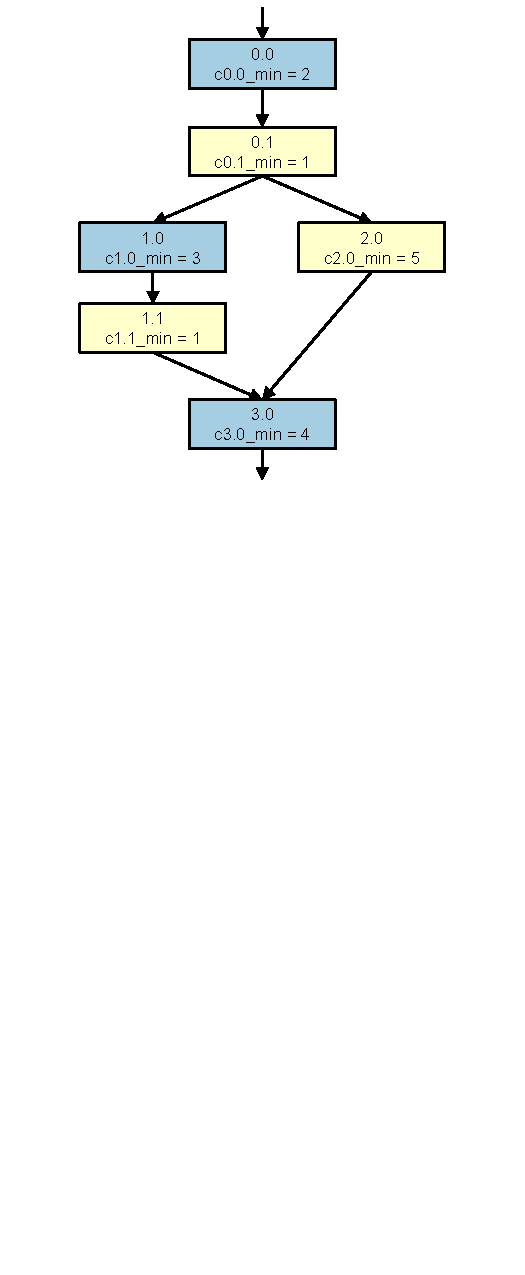
\includegraphics[width=2.9in]{monitoring_wcet/figs/mfg.pdf}
      \label{fig:monitoring_wcet.wcet.mfg} 
    }
    \end{subfigure}
  \end{center} 
  \caption{Example control flow graph and its corresponding monitoring flow
  graph. Blue (dark) nodes include a forwarded instruction.}
  \label{fig:monitoring_wcet.wcet.flow_graphs} 
\end{figure}

In this approach, the original control flow graph must be transformed so that
each node contains at most one forwarded instruction which is located at the
end of the code sequence represented by the node.  This transformed graph is
called a {\em monitoring flow graph (MFG)} (see
Figure~\ref{fig:monitoring_wcet.wcet.flow_graphs}).  Intuitively, the analysis
needs to
consider one forwarded instruction at a time in order to model the FIFO state
on each forwarded instruction and capture all potential stalls from monitoring. 

% Monitoring Load
% \begin{figure} 
%   \begin{center} 
%     \begin{subfigure}[Monitoring load associated with nodes.]{
%       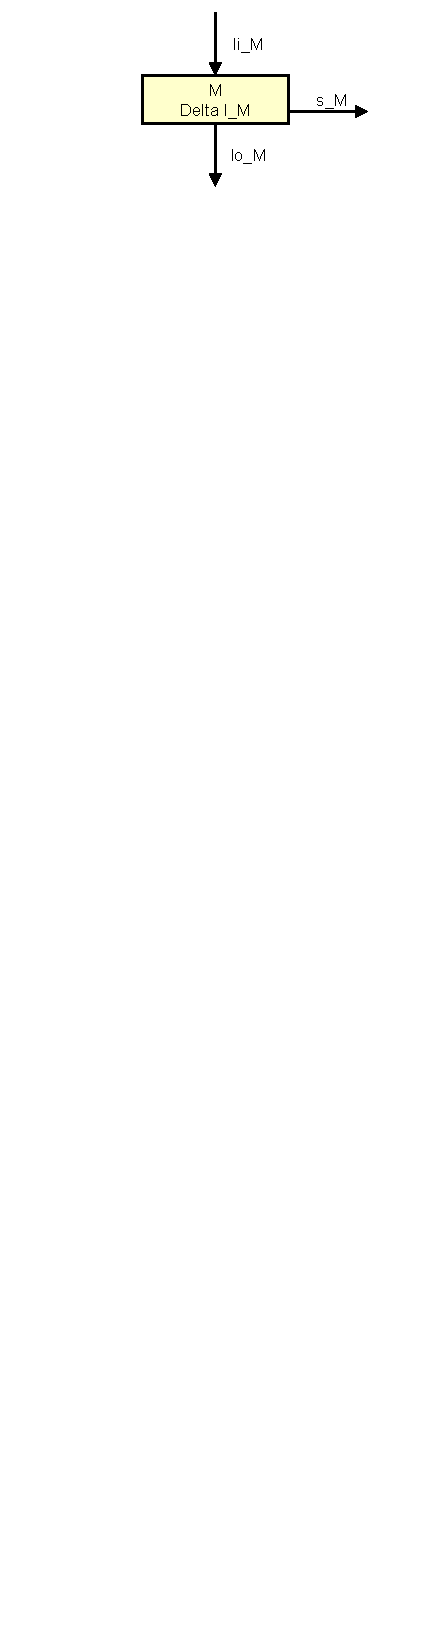
\includegraphics[width=2.9in]{monitoring_wcet/figs/monitoring_load.pdf} 
%       \label{fig:monitoring_wcet.wcet.monitoring_load} 
%     }
%     \end{subfigure}
%     \hspace{-0.3in}
%     \begin{subfigure}[Block diagram of monitoring load model.]{
%       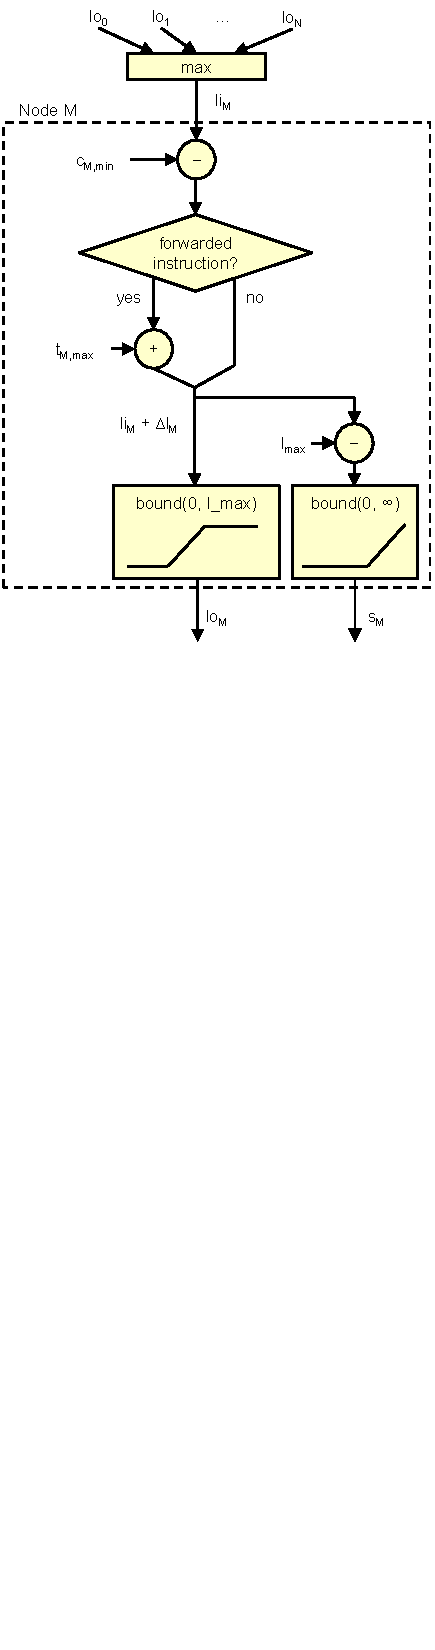
\includegraphics[width=2.9in]{monitoring_wcet/figs/monitoring_load_detailed.pdf}
%       \label{fig:monitoring_wcet.wcet.monitoring_load_detailed} 
%     }
%     \end{subfigure}
%   \end{center} 
%   \caption{Monitoring load is modeled for each node.}
%   \label{fig:monitoring_wcet.wcet.flow_graphs} 
% \end{figure}
\begin{figure}
  \begin{center}
    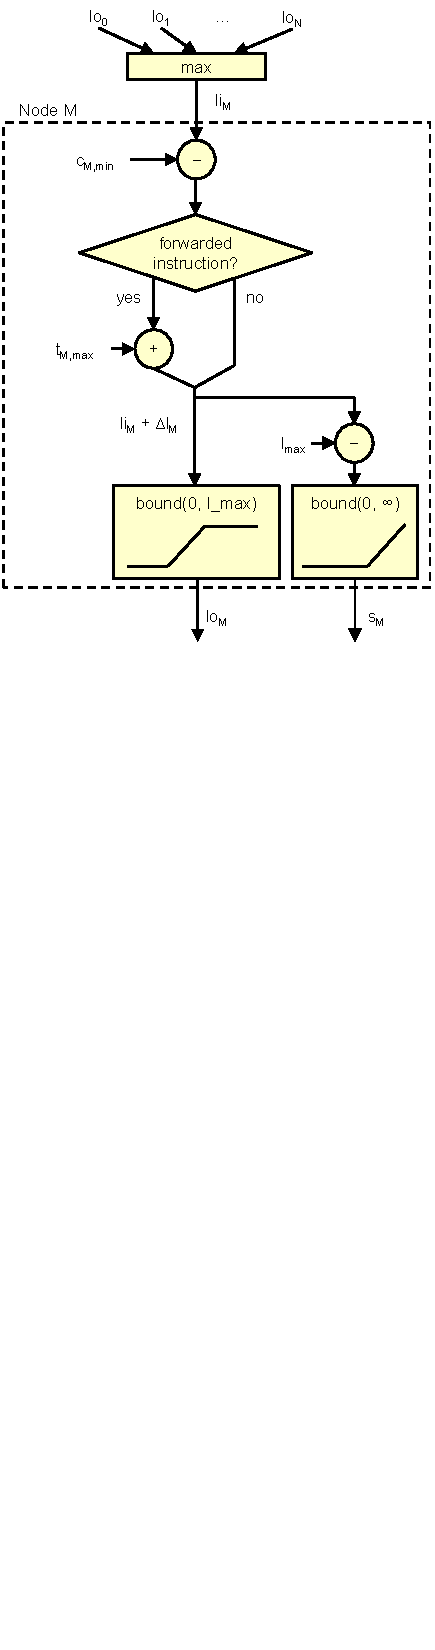
\includegraphics{monitoring_wcet/figs/monitoring_load_detailed.pdf}
    \caption{Monitoring load is modeled for each node.}
    \label{fig:monitoring_wcet.wcet.monitoring_load_detailed}
  \end{center}
\end{figure}

To model how full the FIFO is, we define the concept of \emph{monitoring load}.
The monitoring load is the number of cycles required for the monitoring core to
process all outstanding entries in the FIFO at a given point in time. We model
the input ($li_M$), output ($lo_M$), and change ($\Delta l_M$) in monitoring
load for each node $M$. These are used to
calculate the worst-case stall cycles ($s_M$) for each node.
Figure~\ref{fig:monitoring_wcet.wcet.monitoring_load_detailed} shows a block
diagram of the model for monitoring load which this section will describe in
detail. 

Monitoring load increases when a new instruction is forwarded by the main task,
and decreases as the monitoring core processes forwarded instructions. For
simplicity, the increase in monitoring load for any forwarded instruction is
conservatively assumed to be the worst-case (maximum) monitoring task execution
time among all possible forwarded instructions. This maximum, $t_{M, max}$, can
be obtained from the WCET analysis of the monitoring tasks.  We make this
simplification because it is difficult to model the FIFO mathematically at an
entry-by-entry level. With this simplification, each FIFO entry is identical
and so the monitoring load fully represents the state of the FIFO.  The
monitoring load cannot be negative and is upper-bounded by the maximum
monitoring load the FIFO can handle, $l_{max}$. The maximum monitoring load is
the number of FIFO entries, $n_F$, multiplied by the increase in monitoring
load for one forwarded instruction, $t_{M, max}$.

In order to find the worst-case monitoring stalls, we need to determine the
worst-case (maximum) monitoring load at the node boundaries in the MFG. For a
given node, $M$, in the MFG, we define $li_{M}$ as the monitoring load coming
into the node and $lo_{M}$ as the monitoring load exiting the node. The change
in monitoring load for the node is denoted by $\Delta l_{M}$. The maximum
$\Delta l_{M}$ can be calculated as the difference between the WCET of a
monitoring task that corresponds to $M$ and the minimum execution cycles of the
node, $c_{M,min}$: 
\begin{align*}
\Delta l_{M} = 
	\begin{cases}
	t_{M,max} - c_{M,min}, &\text{forwarded inst. } \in M \\
	- c_{M,min}, &\text{no forwarded inst. } \in M
	\end{cases}
\end{align*}
In order to ensure that the analysis is conservative in estimating the
worst-case (maximum) stalls, we use the best-case (minimum) execution time for
the main task here. 

Because the monitoring load is bounded by zero and the maximum load that
the FIFO can handle, $l_{max}$, the monitoring load coming out of a node is
\begin{align*}
	lo_{M} =& 
		\begin{cases}
			0, &li_{M} + \Delta l_{M} < 0 \\
			li_{M} + \Delta l_{M}, &0 \leq li_{M} + \Delta l_{M} \leq l_{max} \\
			l_{max}, &li_{M} + \Delta l_{M} > l_{max}
		\end{cases} \\
  l_{max} =& n_F \cdot t_{M,max}
\end{align*}

The worst-case monitoring load entering node $M$, $li_{M}$, is the largest of
the output monitoring loads among nodes with edges pointing to node $M$. Let
$\mathcal{M_{\text{prev}}}$ represent the set of nodes with edges pointing to
node $M$. Then,
\begin{align*}
	li_{M} = \max_{M_{prev} \in \mathcal{M}_{prev}}lo_{M_{prev}}
\end{align*}

The above equations describe the worst-case monitoring load at each node
boundary.  A monitoring stall occurs when a forwarded instruction is executed
but there is no empty entry in the FIFO buffer. In terms of monitoring load, if
a node would add monitoring load that would cause the resulting total load to
exceed $l_{max}$, then a monitoring stall occurs. The number of cycles stalled,
$s_{M}$, is the number of cycles that this total exceeds $l_{max}$. That is,
\begin{align*}
	s_{M} =
		\begin{cases}
			0, &li_{M} + \Delta l_{M} < l_{max} \\
			(li_{M} + \Delta l_{M}) - l_{max}, &li_{M} + \Delta l_M \geq l_{max}
		\end{cases}
\end{align*}

These sets of equations describe the monitoring stalls for each node in the MFG.
The worst-case monitoring stall cycles can then be determined by maximizing the
value of each $s_M$. This is equivalent to a single objective of maximizing the
sum of the $s_M$,
\begin{align*}
  \max \sum_{M \in \mathcal{M}_{MFG}} s_{M}
\end{align*}
where $\mathcal{M}_{MFG}$ is the set of nodes in the MFG.  Once the worst-case
stalls for each MFG node is found, the worst-case stalls for a CFG node,
$s_{B,max}$, can be computed by simply summing the stalls from the
corresponding MFG nodes. We note that since the monitoring load is always
conservative in representing the FIFO state, no timing anomalies are exhibited
by this analysis. That is, determining the individual worst-case stalls results
in the global worst-case stalls.

\subsection{MILP Formulation}
\label{sec:monitoring_wcet.wcet.milp}

The proposed FIFO model requires solving an optimization problem to obtain the
worst-case stalls, where the input and output monitoring loads, $li_{M}$ and
$lo_{M}$, and the monitoring stalls, $s_{M}$, need to be determined for each
node. Here, we show how the problem can be formulated using MILP. Although the
equations for $lo_{M}$ and $s_{M}$ are non-linear, they are piecewise linear.
Previous work has shown that linear constraints for piecewise linear functions
can be formulated using MILP \cite{sierksma-lp}. In the following constraints,
all variables are assumed to be lower bounded by zero unless otherwise
specified, as is typically assumed for MILP.

First, a set of variables, $lo'$ and $s'$, are created to represent the
unbounded versions of $lo$ and $s$. For readability, the per block subscript
$M$ has been omitted.
\begin{align*}
  s' =& li + \Delta l - l_{max}, \text{ } s' \in (-\infty, \infty)\\
  lo' =& li + \Delta l, \text{ } lo' \in (-\infty, \infty) 
\end{align*}
The following piecewise linear function calculates $s$ from $s'$.
\begin{align*}
  s = f(s') = 
    \begin{cases} 
    0, &s' < 0\\
    s', &s' \geq 0
    \end{cases}
\end{align*}
This function can be described in MILP using the following set of constraints.
\begin{align*}
  a_s\lambda_0 + b_s\lambda_2 =& s'\\
  \lambda_0 + \lambda_1 + \lambda_2 =& 1 \\
  \delta_1 + \lambda_2 \leq& 1 \\
  \delta_2 + \lambda_0 \leq& 1 \\
  \delta_1 + \delta_2 =& 1 \\
  b_s\lambda_2 =& s
\end{align*}
where $a_s$ is chosen to be less than the minimum possible value of $s'$ and
$b_s$ is chosen to be greater than the maximum possible value of $s'$. The
choice of $a_s$ and $b_s$ is arbitrary as long as it meets these requirements.
$\lambda_i$ are continuous variables and $\delta_i$ are binary variables. In
this set of constraints, $s'$ is expressed as a sum of the endpoints of a
segment of the piecewise function. The $\delta_i$ variables ensure that only
the segment corresponding to $s'$ is considered. $\delta_1 = 1$ corresponds to
the $s' < 0$ segment of $f(s')$ and $\delta_2 = 1$ corresponds to the $s' \geq
0$ segment of $f(s')$. The $\lambda_i$ variables represent exactly where $s'$
falls on the domain of that segment. $s$ can be calculated using this
information and the values of the function at the segment endpoints.

Similarly, $lo$ can be bound between $0$ and $l_{max}$ by using the following
set of constraints.
\begin{align*}
  a_l\lambda_3 + l_{max}\lambda_5 + b_l\lambda_6 =& lo'\\
  \lambda_3 + \lambda_4 + \lambda_5 + \lambda_6 =& 1 \\
  2 \delta_3 + \lambda_5 + \lambda_6 \leq& 2 \\
  2 \delta_4 + \lambda_3 + \lambda_6 \leq& 2 \\
  2 \delta_5 + \lambda_3 + \lambda_4 \leq& 2 \\
  \delta_3 + \delta_4 + \delta_5 = 1 \\
  l_{max}\lambda_5 + l_{max}\lambda_6 =& lo
\end{align*}
As before, $a_l$ and $b_l$ are chosen such that $lo' \in (a_l, b_l)$.  Again,
$\lambda_i$ are continuous variables and $\delta_i$  are binary variables.

Finally, for each node, the input monitoring load $li_{M}$ must be determined.
$li_{M}$ depends on the previous nodes, $\mathcal{M_\text{prev}}$. If there is
only one edge into the node, then $li_M$ is simply
\begin{align*}
  li_{M} = lo_{M_{prev}}
\end{align*}
When there is more than one edge into node $M$, one set of constraints is used
to lower bound $li_{M}$ by all $lo_{M_{prev}}$.
\begin{align*}
  li_{M} \geq& lo_{M_{prev}}, \text{ } \forall M_{prev} \in \mathcal{M_\text{prev}}
\end{align*}
Then, another set of constraints upper bounds $li_{M}$ by the maximum $lo_{M_{prev}}$.
\begin{align*}
  li_{M} - b \cdot \delta_{M_{prev}} \leq& lo_{M_{prev}}, \text{ } \forall M_{prev} \in \mathcal{M_\text{prev}} \\
  \sum_{M_{prev} \in \mathcal{M_\text{prev}}}\delta_{M_{prev}} =& |\mathcal{M_\text{prev}}| - 1
\end{align*}
where $b$ is chosen to be greater than $[\max(lo_{M_{prev}}) -\\
\min(lo_{M_{prev}})]$ and $|\mathcal{M_\text{prev}}|$ is the number of nodes
with edges pointing to $M$. $\delta_i$ are binary variables. The use of the
binary variables $\delta_i$ and the second constraint ensure that $li_{M}$ is
only upper bound by one of the $lo_{M_{prev}}$. In order for all constraints to
hold, this must be the maximum $lo_{M_{prev}}$. Together with the lower bound
constraints, these constraints result in $li_{M} = \max(lo_{M_{prev}})$. 

